\documentclass[11pt, a4paper]{article}

\usepackage[T1]{fontenc}
\usepackage[utf8]{inputenc}
\usepackage[polish]{babel}
\usepackage{listings}
\usepackage{mathtools}
\usepackage{blindtext}
\usepackage{scrextend}
\usepackage{graphicx}


\graphicspath{ {./images/} }


\begin{document}

\title{MOwNiT\\Laboratorium 1}
\author{Kacper Janda}
\maketitle

\section{Wartości błędów dla przykładowych wartości}
 

Wyniki pomiarów dla pojedynczej precyzji:
\begin{center}
    \begin{tabular}{| l | l | l | l | l |}
    \hline
    Wartość & Wartość binarna & Błąd bezwzględny & Błąd względny & Wielkość tablicy\\ \hline
    0.1111111 & 0.000111001 & 102086.875000 & 0.091878 & \begin{math} 10^7 \end{math}\\ \hline
    0.5078125 & 0.1000001 & 76108.500000 & 0.007651 & \begin{math} 10^7 \end{math}\\ \hline
    0.5625000 & 0.1001000 & 508491.500000 & 0.090398 & \begin{math} 10^7 \end{math}\\
    \hline
    \end{tabular}
\end{center}
\vphantom\vphantom\vphantom :Wyniki pomiarów dla podwójnej precyzji:
\begin{center}
    \begin{tabular}{| l | l | l | l | l |}
    \hline
    Wartość & Wartość binarna & Błąd bezwzględny & Błąd względny & Wielkość tablicy\\ \hline
    0.1111111 & 0.000111001 & 0.000182 & 0.000000 & \begin{math} 10^7 \end{math}\\ \hline
    0.5078125 & 0.1000001 & 0.000000 & 0.000000 & \begin{math} 10^7 \end{math} \\ \hline
    0.5625000 & 0.1001000 & 0.000000 & 0.000000 & \begin{math} 10^7 \end{math}\\
    \hline
    \end{tabular}
\end{center}

\vphantom\vphantom\vphantom :Przykładowe dane dające niezerowy błąd względny dla arytmetyki podwójnej precyzji:
\begin{center}
    \begin{tabular}{| l | l | l | l |}
    \hline
    Wartość & Błąd bezwzględny & Błąd względny & Wielkość tablicy\\ \hline
    0.5312523432452345 & 45476.014320 & 0.000001 & \begin{math} 10^{11} \end{math}\\ \hline
    \end{tabular}
\end{center}
\vphantom\vphantom
Użycie podwójnej precyzji zapewnia znaczne bardziej dokładne wyniki ale nie rozwiązuje problemu do końca.\\Błędy numeryczne powstały przez dodawanie dwóch liczb, które znacznie różnią się wielkością. Ich wykładniki muszą zostać sprowadzone do tej samej wartości, co powoduje utratę cyfr znaczących.


\section{Wykresy błędu dla sum cząstkowych}
\vphantom\vphantom
\begin{tabular}{| l | l |} \hline
Wielkość tablicy & \begin{math} 10^7 \end{math}\\ \hline
Wartość & \begin{math} 0.53125 \end{math} \\ \hline
\end{tabular}

\begin{center}
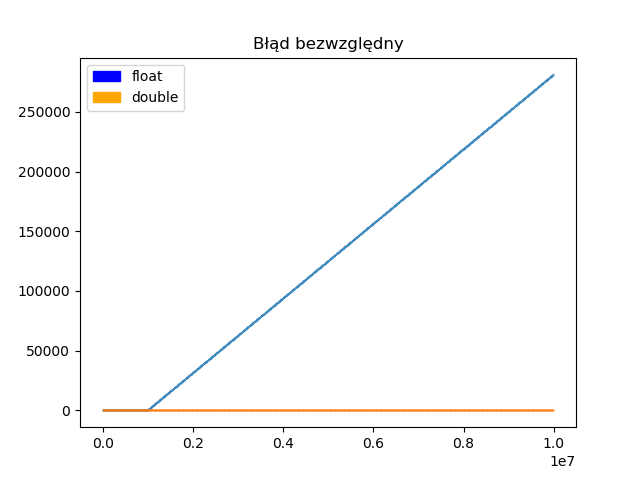
\includegraphics[scale = 0.7]{abs_error_label}\\
\end{center}
\begin{center}
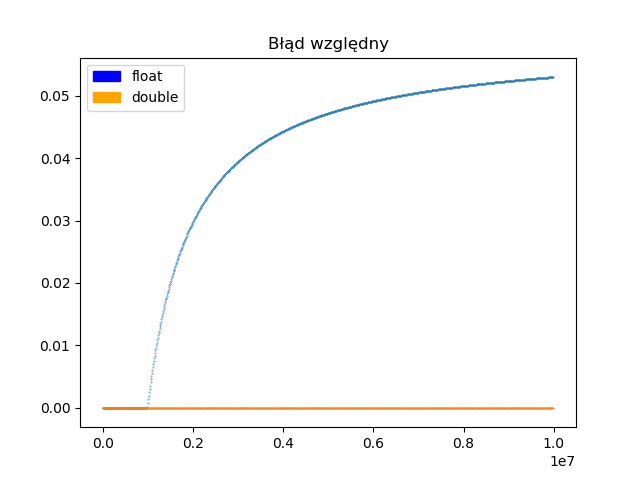
\includegraphics[scale = 0.7]{rel_error_label}\\
\end{center}
Na początku błąd bezwzględny jest równy \begin{math} 0 \end{math}, ponieważ suma jest na tyle mała, że jest możliwe dodanie do niej pojedynczej wartości z pełną dokładnością. Gdy przestaje to być możliwe, błąd względny zaczyna rosnąć. Ponieważ zarówno rzeczywista suma, jak i błąd bezwzględny rosną liniowo lecz ich wykresy nie są do siebie równoległe to wykres błędu względnego jest fragmentem hiperboli.\\


\section{Porównanie wydajności algorytmów}

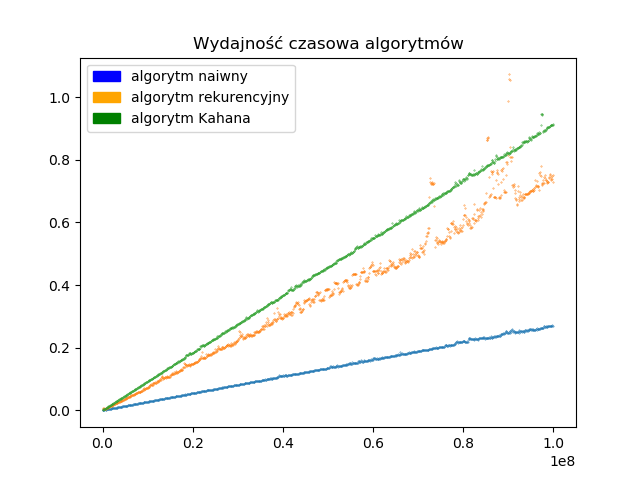
\includegraphics[scale = 0.7]{time_complex}\\
Wraz ze wzrostem dokładności rośnie czas potrzebny do wykonania obliczeń.\\\\ Algorytm Kahana dzięki redukcji błędów numerycznych oraz braku wywołań rekurencyjnych jest najlepszem wyborem jeżeli zależy nam na precyzji obliczeń. Największą zaletą algorytmów naiwnych jest ich szybkość, więc mogą znaleźć zastosowanie w aplikacjach przetwarzających dane w czasie rzeczywistym, w których poprawność numeryczna nie ma najwyższego priorytetu.

\end{document}